\documentclass[conference]{IEEEtran}
\IEEEoverridecommandlockouts
\usepackage[T1]{fontenc}
\usepackage{amsmath,amssymb}
\usepackage{booktabs}
\usepackage{placeins}
\usepackage{flushend}
\usepackage{cite}
\usepackage{tikz}
\usetikzlibrary{arrows.meta}
\definecolor{eventblue}{RGB}{0,92,165}
\definecolor{relationorange}{RGB}{186,83,0}
\definecolor{feedbackpurple}{RGB}{122,58,150}
\definecolor{aggregatecolor}{RGB}{23,94,94}
\usepackage{url}
\usepackage[hidelinks]{hyperref}

\title{TEMPO: Temporal Evidence and Momentum for Market-Neutral Hedging}
\author{\IEEEauthorblockN{Yicheng He\textsuperscript{1,2} and Qianqian Xie\textsuperscript{1,2,*}}
\IEEEauthorblockA{\textsuperscript{1}School of Artificial Intelligence, Wuhan University, Wuhan, China\\
\textsuperscript{2}Cognitive Language and Information Lab, Wuhan University, Wuhan, China\\
Team TEMPO\\
xqq.sincere@gmail.com}
\thanks{\textsuperscript{*}Corresponding author.}}

\begin{document}
\maketitle

\begin{abstract}
We present TEMPO, a market-neutral hedging agent that combines temporal evidence with relative price momentum for FinReason Cup 2026 Task 2. A language model interprets news events and settled forecast errors. Numerical modules represent temporal evidence as time-decaying event, relationship, and feedback factors, integrate their contributions over the prescribed holding interval, and combine their forecasts with observed price movements to select an equal-dollar long--short stock pair or abstain. We evaluate the system retrospectively on 37 rounds with available entry and exit prices from seven public-release dates in October 2026. At a round-trip cost of 10 basis points of account equity, TEMPO earns a cumulative net return of 9.66\% from 30 active rounds, with 1.14\% settlement-endpoint maximum drawdown. Factor-only execution earns 4.67\%. Component ablations yield 3.15\% for price momentum alone, 9.40\% with event factors, and 9.66\% with relationship factors; adding feedback preserves the same actions in this replay. At 20 basis points per round trip, the fixed TEMPO actions earn 6.43\%. In the independent six-round live session on November 2, the fixed method achieves an official return of 2.275\%, nonannualized Sharpe of 1.294, and zero endpoint drawdown, ranking second among participating teams and above all three organizer baselines. This single-session result provides limited prospective evidence.
\end{abstract}

\begin{IEEEkeywords}
financial agents, temporal evidence, price momentum, market-neutral hedging, language models
\end{IEEEkeywords}

\section{Introduction}
FinReason Cup 2026 Task 2 requires repeated decisions from released prices and short news summaries for a fixed stock universe\cite{finreason2026overview,finreason2026task2overview}. A decision can become stale before its position is opened: the current protocol enters at the next valuation node and exits at the following node\cite{task2protocol}. An agent therefore needs to connect the timing of evidence to the interval over which its action is evaluated. HERCULEAN provides the broader financial-agent benchmark context, including hedging as a distinct workflow\cite{peng2026herculeanagenticbenchmarkfinancial}.

We introduce TEMPO: Temporal Evidence and Momentum for Market-Neutral Hedging. TEMPO represents temporal evidence through an append-only collection of signed factors. Each factor has a creation time, an amplitude, a decay family, and a time scale. Its contribution to a prospective holding interval is the amount of remaining influence released during that interval. Factors cover three sources: news events, conditional deviations between related stocks, and forecast errors observed after settlement. The momentum component captures the latest within-session relative price movement, which the decision module combines with the evidence-based forecasts. The language model performs categorical interpretation; deterministic calculations produce forecasts and pair actions.

The retrospective experiments examine how temporal evidence and price momentum contribute to trading returns under delayed execution. We compare TEMPO with factor-only execution and a sentiment--momentum reference, remove factor families to measure their contributions to stock selection, and evaluate sensitivity to the momentum weight and transaction cost. The evaluation uses identical entry and exit prices for every strategy. We then apply the fixed method prospectively to the independently scored November 2 live session and report the official six-round results separately from the October research replay.

\section{Related Work}
Evidence about return reversal depends on the origin and horizon of a price movement. Engelberg, Gao, and Jagannathan associate pairs-trading outcomes with liquidity, common information, and stock-specific news; divergences linked to value-relevant individual news are less favorable for convergence trading\cite{engelberg2008}. Heston, Korajczyk, and Sadka find that quote-based short-term reversals are concentrated at the first half-hour lag, with liquidity recovery taking more than 30 and less than 60 minutes\cite{heston2010}. These findings motivate separate representations for news events and relationship deviations, with each signal evaluated over the task's future holding interval.

Tetlock finds that the market response to stale information differs from the response to new information\cite{tetlock2011}. TEMPO represents the age of an observed event explicitly through its creation time and decay function. The task supplies compressed news summaries, which provide the event model's textual input.

Conditional factor models separate systematic returns from residual deviations\cite{spears2023}. TEMPO's relationship module measures pairwise conditional deviations in the ten-stock universe. It uses a Ledoit--Wolf shrinkage covariance estimate\cite{ledoit2004} to set regression coefficients, correlation eligibility, and residual-volatility thresholds.

Financial prediction from text and prices directly informs TEMPO. The Wall Street Neophyte examines multimodal stock-movement prediction\cite{xie2023wallstreet}, while retrieval-augmented financial time-series forecasting studies how external information enters a numerical forecast\cite{xiao2025retrieval}. TimeLitmus tests whether event-conditioned time-series predictions use both event text and price history, and whether explanations faithfully reflect that evidence\cite{gong2026timelitmus}. TEMPO turns released news into time-stamped factors and combines their holding-interval forecasts with observed price momentum; its experiments evaluate the resulting trading outcomes.

Pair-trading research addresses stock selection and risk-aware sequential decisions\cite{han2023selecttrade,han2023riskpair}. FinCon, InvestorBench, FLAG-Trader, ShiJianBench, and FinCUABuild study financial agents, investment decisions, and evaluation under interactive settings\cite{yu2024fincon,li2025investorbench,xiong2025flagtrader,gong2026shijian,yang2026fincua}. TEMPO tests a fixed pair-action rule under delayed entry and a prescribed exit, with the October replay and November live session reported separately.

Xie and collaborators also provide financial models and evaluation resources through PIXIU, FinBen, Open-FinLLMs, multilingual and multimodal benchmarks, financial expertise tests, reasoning, and structured extraction\cite{xie2023pixiu,xie2024finben,xie2024openfinllms,hu2024nolang,peng2025multifinben,yang2025ucfe,lin2025leaderboard,qian2025fino1,cao2025finaudio,kuang2025scores,wang2025fintagging,zhang2024dolares,peng2025plutus}. Applications in credit scoring, audit, tax practice, misinformation detection, financial simulation, and shared-task design further characterize the domain's evidence and evaluation needs\cite{feng2023credit,huang2024auditwen,huang2026auditjudg,hu2026taxpraben,liu2025fmdllama,liu2025misinformation,liu2026simulation,xie2024agentScen}.

\section{Task, Data, and Temporal Access}
\subsection{Decision and settlement protocol}
The universe is NVDA, GOOG, META, MSFT, JPM, AMZN, AAPL, AMD, WMT, and TSLA. For round $t$, let $p_t$ denote the actual publication time, and let $e_t$ and $x_t$ denote the scheduled entry and exit times. Let $P_{i,u}$ be the published valuation price of stock $i$ at time $u$. TEMPO reads only the release at $p_t$ and previous releases. An active action allocates half of equity to a long stock $L_t$ and half to a short stock $S_t$. Its gross return is
\begin{equation}
 R_t^{\mathrm{gross}}=\tfrac12\left(
 \frac{P_{L_t,x_t}}{P_{L_t,e_t}}-
 \frac{P_{S_t,x_t}}{P_{S_t,e_t}}\right).
\end{equation}
The local research objective uses
\begin{equation}
 R_t^{\mathrm{net}}=R_t^{\mathrm{gross}}-c,
 \qquad c=0.001,
\end{equation}
for an active round; a flat round has zero return and zero cost. The local replay charges ten basis points of account equity for the complete pair round trip. The policy also requires an additional predicted-return margin of five basis points.

All times retain their time-zone offsets. A forecast error becomes eligible only when the exit-price release has been published. Missing terminal prices exclude an interval from evaluation and feedback.

\subsection{Public releases and historical prices}
The October research snapshot contains 41 releases across October 14, 15, 19, 20, 21, 22, and 23, 2026. There are 410 ticker summaries. Of the 41 decision rounds, 37 have both prescribed valuation nodes in the public price files. The four remaining rounds are 11, 12, 40, and 41; their terminal valuation prices are outside the released snapshot. They can produce a prospective action but contribute neither a measured return nor a feedback target.

The supplied news includes 30--50-token English summaries, retrieved-article counts, coverage metadata, and source lists. The event model receives the summary and retrieved count for each ticker; the metadata identifies partial coverage.

For numerical calibration, we use cached Yahoo Finance hourly-bar opens on 709 complete trading dates from December 4, 2023, through October 13, 2026. Each date supplies six common nodes at 09:30, 10:30, 11:30, 12:30, 14:30, and 15:30 New York time. The 3,545 within-session log-return vectors are divided by the square root of their elapsed hours before covariance estimation. Overnight returns are excluded from this covariance fit. These historical bars determine volatility and covariance parameters; replay returns use the competition's published valuation prices.

The replay verifies release identifiers, timestamps, publication deadlines, and available file hashes. The historical calibration ends before the first competition release, and feedback uses only outcomes released by the current decision time.

\section{TEMPO Architecture}
At each release, TEMPO evaluates newly settled forecasts and appends any accepted feedback factors. It then creates relationship and event factors from the released prices and news. These factors encode temporal evidence and produce forecasts for the scheduled holding interval. The decision module combines the forecasts with relative price momentum to choose a pair or abstain. Fig.~\ref{fig:architecture} shows the information flow.

\begin{figure*}[t]
\centering
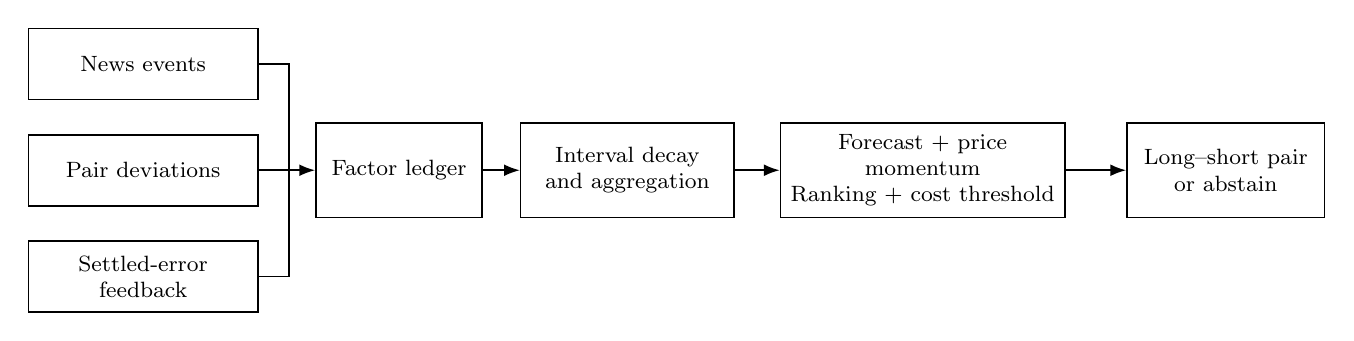
\begin{tikzpicture}[
  box/.style={draw, line width=0.6pt, align=center, minimum height=9mm,
              inner sep=3pt, font=\footnotesize},
  source/.style={box, text width=2.7cm},
  stage/.style={box, minimum height=12mm},
  flow/.style={-{Latex[length=2mm]}, line width=0.6pt}
]
\node[source] (events) at (1.55,1.35) {News events};
\node[source] (relations) at (1.55,0) {Pair deviations};
\node[source] (feedback) at (1.55,-1.35) {Settled-error feedback};

\node[stage, text width=1.9cm] (ledger) at (4.8,0) {Factor ledger};
\node[stage, text width=2.5cm] (interval) at (7.7,0) {Interval decay\\and aggregation};
\node[stage, text width=3.4cm] (decision) at (11.45,0) {Forecast + price momentum\\Ranking + cost threshold};
\node[stage, text width=2.3cm] (action) at (15.3,0) {Long--short pair\\or abstain};

\draw[line width=0.6pt] (events.east) -- (3.4,1.35) -- (3.4,-1.35) -- (feedback.east);
\draw[line width=0.6pt] (relations.east) -- (3.4,0);
\draw[flow] (3.4,0) -- (ledger.west);
\draw[flow] (ledger.east) -- (interval.west);
\draw[flow] (interval.east) -- (decision.west);
\draw[flow] (decision.east) -- (action.west);
\end{tikzpicture}
\caption{TEMPO workflow.}
\label{fig:architecture}
\end{figure*}

\subsection{Temporal evidence and interval contribution}
A factor $k$ stores its stock $i(k)$, creation time $p_k$, signed amplitude $A_k$, time scale $\tau_k>0$, and family $z_k$. Creation time is the time the release becomes available to the agent. Amplitudes and signs are immutable after creation. With elapsed wall-clock hours $u\geq0$, the remaining-influence functions are
\begin{align}
 S_{\mathrm{event}}(u;\tau)&=\exp[-(u/\tau)^{0.75}],\\
 S_{\mathrm{relation}}(u;\tau)&=\exp(-u/\tau),\\
 S_{\mathrm{feedback}}(u;\tau)&=(1+u/\tau)^{-1.5}.
\end{align}
The factor's predicted return contribution is
\begin{equation}
 v_{k,t}=A_k\left[S_{z_k}(e_t-p_k;\tau_k)
                    -S_{z_k}(x_t-p_k;\tau_k)\right].
 \label{eq:interval}
\end{equation}
The time differences in \eqref{eq:interval} are expressed in hours. Each survival function decreases, so an individual contribution retains its original sign. Eq.~\eqref{eq:interval} measures the remaining response between entry and exit, and wall-clock aging continues overnight. Fig.~\ref{fig:factor_decay} illustrates the factor-to-forecast calculation.

The three decay families express different persistence assumptions. The stretched exponential gives an event a sharp early response and a slower later tail; the exponential assigns a single characteristic scale to a relationship deviation; the power law allows feedback from a settled forecast error to persist longer. These functional forms and their exponents are modeling choices, not estimates identified by the 37-round sample. Their half-lives are $\tau(\ln 2)^{4/3}$, $\tau\ln 2$, and $\tau(2^{2/3}-1)$, respectively. We use elapsed wall-clock time because the next entry and exit times are fixed by the protocol.

\begin{figure*}[t]
\centering
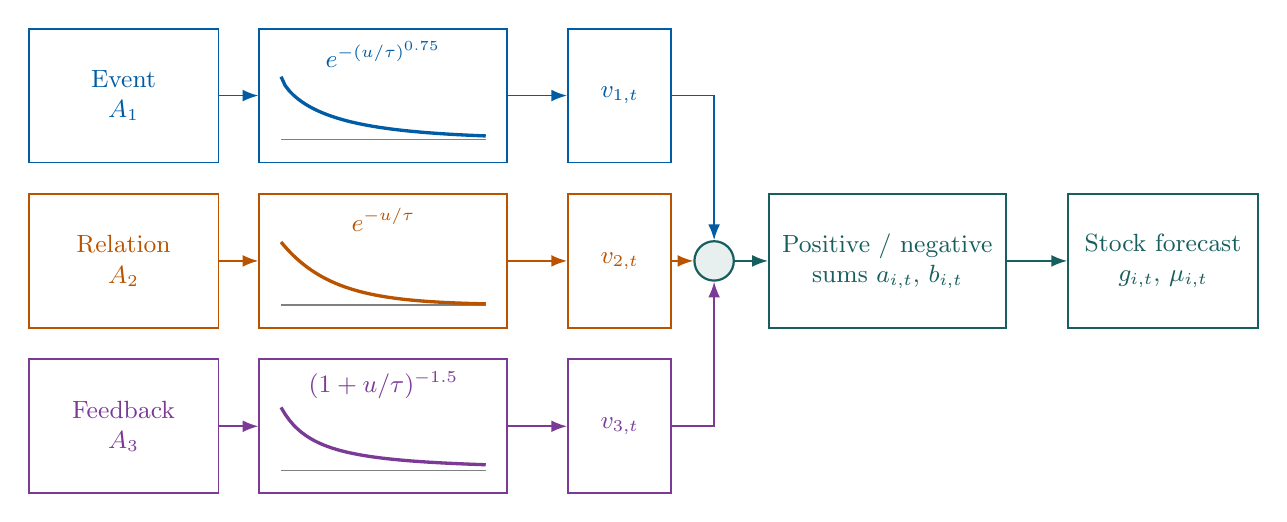
\begin{tikzpicture}[
  factorbox/.style={draw, line width=0.7pt, align=center, minimum height=17mm,
                    text width=2.2cm, inner sep=3pt, font=\small},
  curvebox/.style={draw, line width=0.7pt, minimum width=3.15cm,
                   minimum height=17mm},
  valuebox/.style={draw, line width=0.7pt, minimum height=17mm,
                   text width=1.1cm, align=center, inner sep=3pt, font=\small},
  resultbox/.style={draw, line width=0.6pt, minimum height=17mm,
                    align=center, inner sep=3pt, font=\small},
  flow/.style={-{Latex[length=2mm]}, line width=0.6pt}
]
\node[factorbox, draw=eventblue, text=eventblue] (event) at (1.35,2.1) {Event\\$A_1$};
\node[factorbox, draw=relationorange, text=relationorange] (relation) at (1.35,0) {Relation\\$A_2$};
\node[factorbox, draw=feedbackpurple, text=feedbackpurple] (feedback) at (1.35,-2.1) {Feedback\\$A_3$};

\node[curvebox, draw=eventblue] (sevent) at (4.65,2.1) {};
\node[curvebox, draw=relationorange] (srelation) at (4.65,0) {};
\node[curvebox, draw=feedbackpurple] (sfeedback) at (4.65,-2.1) {};
\node[font=\small, text=eventblue] at (4.65,2.62) {$e^{-(u/\tau)^{0.75}}$};
\node[font=\small, text=relationorange] at (4.65,0.52) {$e^{-u/\tau}$};
\node[font=\small, text=feedbackpurple] at (4.65,-1.58) {$(1+u/\tau)^{-1.5}$};
\draw[line width=0.4pt, draw=black!50] (3.35,1.54) -- (5.95,1.54);
\draw[line width=0.4pt, draw=black!50] (3.35,-0.56) -- (5.95,-0.56);
\draw[line width=0.4pt, draw=black!50] (3.35,-2.66) -- (5.95,-2.66);
\draw[line width=1.2pt, draw=eventblue, domain=0:2.6, samples=50]
  plot ({3.35+\x},{1.54+0.8*exp(-pow(4*\x/2.6,0.75))});
\draw[line width=1.2pt, draw=relationorange, domain=0:2.6, samples=50]
  plot ({3.35+\x},{-0.56+0.8*exp(-4*\x/2.6)});
\draw[line width=1.2pt, draw=feedbackpurple, domain=0:2.6, samples=50]
  plot ({3.35+\x},{-2.66+0.8*pow(1+4*\x/2.6,-1.5)});

\node[valuebox, draw=eventblue, text=eventblue] (v1) at (7.65,2.1) {$v_{1,t}$};
\node[valuebox, draw=relationorange, text=relationorange] (v2) at (7.65,0) {$v_{2,t}$};
\node[valuebox, draw=feedbackpurple, text=feedbackpurple] (v3) at (7.65,-2.1) {$v_{3,t}$};
\node[circle, draw=aggregatecolor, fill=aggregatecolor!10,
      minimum size=5mm, inner sep=0pt, line width=0.8pt] (merge) at (8.85,0) {};
\node[resultbox, draw=aggregatecolor, text=aggregatecolor,
      text width=2.8cm] (sums) at (11.05,0)
  {Positive / negative\\sums $a_{i,t},\,b_{i,t}$};
\node[resultbox, draw=aggregatecolor, text=aggregatecolor,
      text width=2.2cm] (forecast) at (14.55,0)
  {Stock forecast\\$g_{i,t},\,\mu_{i,t}$};

\draw[flow, draw=eventblue] (event.east) -- (sevent.west);
\draw[flow, draw=relationorange] (relation.east) -- (srelation.west);
\draw[flow, draw=feedbackpurple] (feedback.east) -- (sfeedback.west);
\draw[flow, draw=eventblue] (sevent.east) -- (v1.west);
\draw[flow, draw=relationorange] (srelation.east) -- (v2.west);
\draw[flow, draw=feedbackpurple] (sfeedback.east) -- (v3.west);
\draw[flow, draw=eventblue] (v1.east) -- (8.85,2.1) -- (merge.north);
\draw[flow, draw=relationorange] (v2.east) -- (merge.west);
\draw[flow, draw=feedbackpurple] (v3.east) -- (8.85,-2.1) -- (merge.south);
\draw[flow, draw=aggregatecolor] (merge.east) -- (sums.west);
\draw[flow, draw=aggregatecolor] (sums.east) -- (forecast.west);
\end{tikzpicture}
\caption{Factor decay and aggregation.}
\label{fig:factor_decay}
\end{figure*}

\subsection{News-event factors}
One language-model request processes all ten stocks per release. The model returns one to three separately described events per ticker. Every event receives one of five levels and one of three response-speed labels. A ticker with no clear directional event receives a single neutral record. For historical hourly volatility $\sigma_i$, the amplitude is
\begin{equation}
 A_k=\ell_k\sigma_{i(k)},\quad
 \ell_k\in\{-2,-0.75,0,0.75,2\}.
\end{equation}
The fast, medium, and slow time scales are $0.5$, $1.5$, and $4$ hours. Event records retain the reason, source round, category, and speed. Each event contributes its own signed interval response, allowing conflicting news to coexist in the same stock forecast.
The corresponding event half-lives are approximately $0.31$, $0.92$, and $2.46$ hours. Discrete volatility-scaled amplitudes prevent the language model from assigning unrestricted numerical returns from short summaries. We evaluated amplitude multipliers $\{0.5,1,2\}$ and three time-scale triplets on the development dates as described in Section~V-A; the shape exponent was held fixed.

\subsection{Relationship-deviation factors}
Let $\Sigma$ be the shrunk hourly covariance matrix, $\rho_{ij}$ its correlation, and $\beta_{ij}=\Sigma_{ij}/\Sigma_{jj}$. For the most recent same-day log-return vector $r_t$ over $h_t$ hours, define
\begin{align}
 d_{ij,t}&=r_{i,t}-\beta_{ij}r_{j,t},\\
 s_{ij,t}&=\sqrt{h_t(\Sigma_{ii}-\Sigma_{ij}\beta_{ij})}.
\end{align}
Pairs are enumerated once in the fixed universe order. A pair is eligible when $\rho_{ij}\geq0.45$ and $|d_{ij,t}|>2s_{ij,t}$. Its total amplitude magnitude is
\begin{equation}
 B_{ij,t}=\rho_{ij}\min\{|d_{ij,t}|-2s_{ij,t},3s_{ij,t}\}.
\end{equation}
We append amplitudes $-\operatorname{sign}(d_{ij,t})B_{ij,t}/2$ for stock $i$ and the opposite for stock $j$, with $\tau=1+4(1-\rho_{ij})$ hours. Relationship factors use within-session observations.
The two amplitudes sum to zero by construction. The $2s$ trigger suppresses small deviations, the $3s$ cap limits the effect of an extreme observation, and the time scale shortens as correlation rises. These thresholds are design assumptions; the present sample does not identify an optimal relationship-decay law.

\subsection{Factor aggregation}
For each stock, collect the positive and negative contributions:
\begin{equation}
 a_{i,t}=\sum_{k:i(k)=i}\max(v_{k,t},0),\qquad
 b_{i,t}=\sum_{k:i(k)=i}\max(-v_{k,t},0).
\end{equation}
We use a uniform return distribution $U[-b_{i,t},a_{i,t}]$ as a scoring representation. It yields
\begin{align}
 g_{i,t}&=\exp\{\mathbb{E}[\log(1+R_{i,t})]\}-1,\\
 \mu_{i,t}&=(a_{i,t}-b_{i,t})/2.
\end{align}
The expected logarithm is computed by 16-point Gauss--Legendre quadrature, with $b_{i,t}<1$ enforced. The factor module provides $g_{i,t}$ for stock ranking and $\mu_{i,t}$ for arithmetic-return calculations.

\subsection{Feedback from settled forecasts}
The feedback rule compares realized stock return $y_{i,t}$ with the factor module's geometric forecast $g_{i,t}$ stored at decision time:
\begin{equation}
 \epsilon_{i,t}=y_{i,t}-g_{i,t}.
\end{equation}
A stock is sent for feedback interpretation only if
$|\epsilon_{i,t}|>2\sigma_i\sqrt{x_t-e_t}$, with duration in hours. This applies to forecasts from both active and flat decisions, provided the required prices have been published. The model sees candidate errors and current summaries, and decides whether to add a factor. Accepted low, medium, and high strengths map to $\alpha\in\{0.25,0.5,1\}$. The factor amplitude is $\alpha\epsilon_{i,t}$ with a three-hour time scale. Its direction follows the observed error, while the model controls whether the error persists in the forecast and at what strength.

The power-law half-life at the three-hour scale is approximately $1.76$ hours. The trigger ties the error threshold to historical volatility and holding duration; the three strengths bound the fraction of an observed error that can be carried forward. Feedback uses raw factor forecasts, released prices, news, and previous factors. The momentum weight and trading threshold therefore leave the factor trajectory unchanged.

\subsection{Momentum and hedging decisions}
For a release with a preceding observation in the same session, define the centered log-price movement across the $N=10$ stocks:
\begin{equation}
 m_{i,t}=\log\frac{P_{i,t}}{P_{i,t-1}}-
 \frac{1}{N}\sum_{j=1}^{N}\log\frac{P_{j,t}}{P_{j,t-1}}.
\end{equation}
At the first observation of a session, $m_{i,t}=0$. The decision policy combines the signals as
\begin{equation}
 q_{i,t}=g_{i,t}+\lambda m_{i,t},\qquad
 \widehat\mu_{i,t}=\mu_{i,t}+\lambda m_{i,t},\quad \lambda=1.5.
\end{equation}
It selects the highest-$q$ stock for the long leg and the lowest-$q$ stock for the short leg. The position is active when the stocks differ and
\begin{equation}
 \tfrac12(\widehat\mu_{L_t,t}-\widehat\mu_{S_t,t})-0.001>0.0005.
\end{equation}
Otherwise, it abstains. Setting $\lambda=0$ gives the factor-only execution reference. The price term uses the most recent observed move, while each event term carries its remaining response over the future entry-to-exit interval. Both enter the same deterministic stock-selection and cost-threshold calculation.

\begin{table*}[!t]
\centering
\caption{Trading performance on 37 evaluable rounds at 10 bps per active pair round trip. Returns and drawdowns are percentages; Sharpe is not annualized.}
\label{tab:performance}
\begin{tabular}{lrrrrrr}
\toprule
Configuration & Development & Later dates & All dates & Active rounds & Sharpe & Max. drawdown\\
\midrule
TEMPO & 6.658 & 2.813 & 9.658 & 30 & 0.312 & 1.142\\
Factor-only execution & 4.103 & 0.548 & 4.673 & 7 & 0.305 & 0.149\\
FinBERT + momentum reference & 2.140 & 2.957 & 5.160 & 37 & 0.200 & 2.284\\
\bottomrule
\end{tabular}
\end{table*}

\section{Experiments}
\subsection{Evaluation protocol}
October 14, 15, 19, and 20 form the four-date development partition, containing 22 evaluable rounds. October 21--23 form a later-date partition containing 15 evaluable rounds. Configuration selection maximizes development net cumulative return. Both partitions were used during architecture development; their separate returns describe temporal variation within the research sample.

Factor calibration covers nine event-only combinations: amplitude multipliers $\{0.5,1,2\}$ applied to the levels in Section IV-B and time-scale triplets $(0.5,1.5,4)$, $(1,3,8)$, and $(2,6,16)$ hours. Feedback calibration compares errors relative to geometric forecasts, arithmetic forecasts, and cross-sectionally centered arithmetic forecasts. The resulting factor parameters are those specified in Section IV.

The adaptively expanded execution search covers 15 configurations: four factor-only margins of 0, 2.5, 5, and 10 basis points (bps); five momentum weights of 0.25, 0.5, 1, 1.5, and 2 at a 5-bps margin; three additional margins of 0, 2.5, and 10 bps at weight 1; and three online ridge penalties of 1, 10, and 100 at a 5-bps margin. The online candidates regress centered realized stock returns on centered arithmetic forecasts and price movements, with all values divided by 0.01 and coefficients regularized toward $(1,0)$. They use only outcomes whose exit prices have been published. Weights 1.5 and 2 share the highest development return and produce identical evaluable actions. TEMPO uses weight 1.5.

All execution configurations use the same recorded factor trajectory. For component ablations, we retain the specified factor families and recompute their forecasts and trading actions at the fixed weight of 1.5 and margin of 5 bps. Entry prices, exit prices, and evaluable rounds are identical across comparisons. Cumulative return is $\prod_t(1+R_t^{\mathrm{net}})-1$. Sharpe is the mean completed-round return divided by its sample standard deviation, including flat rounds and with no annualization. Maximum drawdown is measured at settlement endpoints, including initial equity of one.

\subsection{Trading performance}
Table~\ref{tab:performance} compares TEMPO with two reference strategies. Factor-only execution sets $\lambda=0$ while preserving all three factor types and the 5-bps margin. The FinBERT + momentum reference combines positive-minus-negative FinBERT sentiment\cite{araci2019} with the latest same-day log return, centered by its cross-sectional median and divided by 0.01. It selects extremes among stocks with retrieved news; when a same-day price difference is unavailable, it uses sentiment alone.

TEMPO earns 9.66\% cumulative net return, exceeding factor-only execution by 4.98 percentage points. Its development return is 6.66\%, and its later-date return is 2.81\%. Trading activity rises from seven to 30 rounds relative to factor-only execution, while endpoint maximum drawdown rises from 0.15\% to 1.14\%. Five of the seven date-level returns improve. The FinBERT + momentum reference earns 5.16\% over all dates and 2.96\% on the later dates, with 37 active rounds and 2.28\% endpoint maximum drawdown over the full replay.

\subsection{Momentum-weight sensitivity}
Table~\ref{tab:execution} varies the momentum weight while holding the factor trajectory and 5-bps margin fixed. At weight 0.25, cumulative return is 1.65\%; at weights 1.5 and 2, it is 9.66\%. Weights 1, 1.5, and 2 have identical later-date returns, with the development-date stock selections distinguishing weight 1 from the two larger weights.

\begin{table}[!tb]
\centering
\caption{Momentum-weight sensitivity at a fixed 5-bps margin and 10-bps cost. Returns are percentages.}
\label{tab:execution}
\begin{tabular}{rrrrr}
\toprule
Weight & Development & Later & All & Active rounds\\
\midrule
0 & 4.103 & 0.548 & 4.673 & 7\\
0.25 & 1.183 & 0.463 & 1.652 & 20\\
0.5 & 4.955 & 0.458 & 5.436 & 26\\
1 & 6.223 & 2.813 & 9.210 & 30\\
1.5 & 6.658 & 2.813 & 9.658 & 30\\
2 & 6.658 & 2.813 & 9.658 & 30\\
\bottomrule
\end{tabular}
\end{table}

\subsection{Contribution of price and evidence factors}
At momentum weight 1.5 and the fixed cost threshold, price momentum alone earns 3.15\%. Adding event factors raises return to 9.40\%; adding relationship factors raises it to 9.66\% (Table~\ref{tab:components}). All four component settings trade in the same 30 rounds, so these differences arise from the selected stocks. Feedback factors preserve the same evaluable actions after the event and relationship terms are present. The return contribution of event and relationship factors occurs in the development partition; all four settings have the same later-date return.

\begin{table}[!tb]
\centering
\caption{Decision inputs at momentum weight 1.5 and a 5-bps margin. Returns are percentages.}
\label{tab:components}
\begin{tabular}{lrrr}
\toprule
Inputs & Development & Later & All\\
\midrule
Price & 0.328 & 2.813 & 3.150\\
Price + events & 6.406 & 2.813 & 9.399\\
Price + events + relationships & 6.658 & 2.813 & 9.658\\
All three factor types + price & 6.658 & 2.813 & 9.658\\
\bottomrule
\end{tabular}
\end{table}

\subsection{Cost and date sensitivity}
Table~\ref{tab:cost} varies the realized cost while retaining TEMPO's actions and decision threshold. Cumulative net return is 9.66\% at 10 bps and 6.43\% at 20 bps per active round. For date sensitivity, we keep the recorded feedback trajectory and remove one date's scored returns at a time. Cumulative return across the seven deletion cases ranges from 6.57\% to 9.85\%.

\subsection{Market-beta exposure}
We estimate each stock's beta against the SPY exchange-traded fund using matched historical Yahoo Finance hourly-bar opens. The 3,490 within-session intervals span 698 complete dates from December 19, 2023, through October 13, 2026, all before the first competition release. As in the covariance calibration, log returns are divided by the square root of elapsed hours. Ordinary least squares gives $\widehat\beta_i=\operatorname{Cov}(r_i,r_{\mathrm{SPY}})/\operatorname{Var}(r_{\mathrm{SPY}})$; the equal-dollar pair has estimated beta $(\widehat\beta_L-\widehat\beta_S)/2$. Among the 30 active evaluable replay pairs, mean absolute beta is $0.488$, median absolute beta is $0.479$, and maximum absolute beta is $0.907$. The five active live pairs have mean absolute beta $0.568$ and maximum absolute beta $0.907$. Equal-dollar allocation therefore leaves material estimated market exposure. SPY is a market proxy, and these historical estimates do not measure realized intrainterval exposure.

\begin{table}[!tb]
\centering
\caption{TEMPO sensitivity to pair round-trip costs, with trading actions held fixed.}
\label{tab:cost}
\begin{tabular}{rrr}
\toprule
Cost (bps) & Cumulative return (\%) & Max. drawdown (\%)\\
\midrule
0 & 12.986 & 0.843\\
5 & 11.310 & 0.893\\
10 & 9.658 & 1.142\\
20 & 6.425 & 1.833\\
\bottomrule
\end{tabular}
\end{table}

\section{Implementation and Reproducibility}
The implementation uses the DeepSeek API model identifier \texttt{deepseek-flash}, with thinking disabled and JSON-object output. Event and feedback response limits are 3,200 and 1,600 tokens, respectively. The model is prompted to use only supplied data. Outputs must satisfy ticker order, category, count, and type constraints; invalid responses terminate execution. The replay uses 41 event calls and eight feedback calls, totaling 36,940 prompt tokens and 15,410 completion tokens.

Requests are cached by a SHA-256 digest of the model identifier and complete messages. The cache records response identifiers, returned model identifiers, fingerprints, parsed output, and token usage. The reported execution comparisons reproduce one stored model-response trajectory. Each report records input-file hashes, numerical parameters, factors, predictions, actions, and settlements.

An independent replay reconstructs factor contributions, stock selections, and returns from the published entry and exit prices. At every release, decisions computed from the full stored price array equal those computed from an array truncated at that release. A separate agent run ending at round 25 reproduces the first 25 decisions, factors, and forecasts of the 41-round run. Feedback eligibility is checked against the publication time of each exit-price observation. These checks verify the numerical results and temporal access rules used in the reported replay.

\FloatBarrier
\section{Live Trading}
\subsection{Prospective protocol and fixed configuration}
The third phase comprised six independently scored rounds on November 2, 2026, with starting equity reset to one\cite{task2protocol,task2livefinal}. Scheduled releases ran hourly from 09:30 through 14:30 New York time (EST, UTC$-5$). Each action entered at the next valuation node; the final holding interval was 15:30--16:00. The organizer's final feed, updated at 16:03:14 EST, marks all six rounds verified and the phase finished.

We retained the pre-session TEMPO configuration: \texttt{deepseek-flash} with thinking disabled, the factor parameters in Section IV, momentum weight 1.5, a 10-bps decision-cost allowance, and a 5-bps additional margin. The stored method hashes match the implementation, and all six decision records use the same model and policy. The factor history continued from the October replay, while scoring started afresh for November 2. New factors and eligible feedback were appended as releases arrived. The official action history agrees with the six archived decisions: one flat round followed by five long--short rounds (Table~\ref{tab:live_actions}).

\begin{table}[!tb]
\centering
\caption{TEMPO live actions and available official step returns. Times are New York EST; each pair lists long/short. A dash denotes an individually unavailable return.}
\label{tab:live_actions}
\small
\setlength{\tabcolsep}{3pt}
\begin{tabular}{cllr}
\toprule
Release & Holding interval & Action & Return (\%)\\
\midrule
09:30 & 10:30--11:30 & Flat & 0.000\\
10:30 & 11:30--12:30 & AMZN/AAPL & 0.446\\
11:30 & 12:30--13:30 & WMT/AMD & 0.826\\
12:30 & 13:30--14:30 & WMT/AAPL & 0.162\\
13:30 & 14:30--15:30 & GOOG/AMD & ---\\
14:30 & 15:30--16:00 & WMT/AMD & ---\\
\bottomrule
\end{tabular}
\end{table}

\subsection{Official results and evidence coverage}
Table~\ref{tab:live_results} reports the official final metrics for TEMPO and the three organizer baselines\cite{task2livefinal}. TEMPO earns 2.274751\% cumulative return, with nonannualized Sharpe 1.294271 and zero settlement-endpoint maximum drawdown. It ranks second among participating teams and exceeds Moira, FinMem, and Codex in cumulative return.

\begin{table}[!tb]
\centering
\caption{Official six-round live results for TEMPO and the organizer baselines. Returns and endpoint maximum drawdowns (MDD) are percentages; Sharpe is not annualized.}
\label{tab:live_results}
\begin{tabular}{lrrr}
\toprule
Entry & Return & Sharpe & MDD\\
\midrule
TEMPO & 2.275 & 1.294 & 0.000\\
Moira (baseline) & 1.063 & 0.458 & 0.094\\
FinMem (baseline) & 0.669 & 0.715 & 0.166\\
Codex (baseline) & $-1.517$ & $-0.668$ & 1.707\\
\bottomrule
\end{tabular}
\end{table}

Official metrics use only the six live rounds. Sharpe includes the flat round and uses sample standard deviation and zero risk-free return; maximum drawdown includes initial equity and settlement endpoints\cite{task2protocol}. These are organizer-reported scores; the 10-bps cost used in our research replay and decision threshold is not deducted again. The local report's cumulative result across October and November is excluded from this live evaluation.

For rounds 1--4, consecutive archived official snapshots yield step returns of 0.000000\%, 0.446289\%, 0.825831\%, and 0.162112\%. They independently match the equal-dollar gross returns recomputed from the public valuation prices. The final snapshot supplies aggregate metrics and all six actions, but no exact individual returns for rounds 5--6. Their combined compounded return is 0.822916\%, obtained by dividing final equity by equity after round 4 and subtracting one. The archived public price releases end at 14:30, so the terminal 15:30 and 16:00 prices cannot be independently checked from those files. We retain the published final metrics and report the two individual returns as unavailable.

\subsection{Interpretation and limitations}
The session evaluates decisions made with a method fixed before the releases and documents successful execution of the temporal-access workflow. Its five active decisions cover one trading day and a ten-stock universe. This sample does not establish persistent profitability, statistical superiority, or the live contribution of any individual factor family. Equal-dollar positions have nonzero estimated market beta, and zero endpoint drawdown leaves intrainterval exposure unmeasured. The competition uses simulated valuation and execution; realized brokerage fills, slippage, and financing costs remain outside this result. Longer prospective evaluation with complete settlement data is needed to assess generalization and forecast calibration.

\FloatBarrier
\bibliographystyle{IEEEtran}
\section*{Code and Data Availability}
The implementation, prompts, cached parsed model responses, released inputs, and numerical reports are available at \url{https://github.com/shenma32/TEMPO}.

\bibliography{official-overviews,official-herculean,references,xie-finance}
\end{document}
